% !TeX root = 2021-22-COMP110-08-lecture-materials-screen.tex
% Adjust these for the path of the theme and its graphics, relative to this file
%\usepackage{beamerthemeFalmouthGamesAcademy}
\usepackage{../../beamerthemeFalmouthGamesAcademy}
\usepackage{multimedia}
\graphicspath{ {../../} }

% Default language for code listings
\lstset{language=[Sharp]C
}

% For strikethrough effect
\usepackage[normalem]{ulem}
\usepackage{wasysym}

\usepackage{algpseudocode}

\usepackage{pdfpages}
\usepackage{qtree}

% http://www.texample.net/tikz/examples/state-machine/
\usetikzlibrary{arrows,automata}
\usetikzlibrary{tikzmark,calc}

\newcommand{\modulecode}{COMP260}\newcommand{\moduletitle}{Distributed Systems}\newcommand{\sessionnumber}{5}

\begin{document}
\title{\sessionnumber: Data Structures I}
\subtitle{\modulecode: \moduletitle}

\frame{\titlepage} 

%\begin{frame}
%	\frametitle{Learning outcomes}
%	\begin{itemize}
%		\item \textbf{Explain} the difference between pass-by-value and pass-by-reference
%		\item \textbf{Distinguish} the basic data structures available in Python
%		\item \textbf{Determine} the complexity of accessing and manipulating data in these data structures
%		\item \textbf{Choose} the correct data structure for a given task
%	\end{itemize}
%\end{frame}

\begin{frame}{Administration}
    \begin{itemize}
        \pause\item Research Journal Peer Review is \textbf{today}
        \pause\item Final deadline is \textbf{soon (check MyFalmouth)}
    \end{itemize}
\end{frame}

\part{Basic containers in Python}
\frame{\partpage}

\begin{frame}{Memory allocation}
	\begin{itemize}
		\pause\item Memory is allocated in \textbf{blocks}
		\pause\item The program specifies the size, in bytes, of the block it wants
		\pause\item The OS allocates a \textbf{contiguous} block of that size
		\pause\item The program owns that block until it frees it
		\pause\item Forgetting to free a block is called a \textbf{memory leak}
			(not really possible in Python, but a common bug in C++)
		\pause\item Blocks can be allocated and deallocated at will, but can \textbf{never grow or shrink}
	\end{itemize}
\end{frame}

\begin{frame}{Containers}
	\begin{itemize}
		\pause\item Memory management is hard and programmers are lazy
		\pause\item Containers are an \textbf{abstraction}
			\begin{itemize}
				\pause\item Hide the details of memory allocation, and allow the programmer to write simpler code
			\end{itemize}
		\pause\item Containers are an \textbf{encapsulation}
			\begin{itemize}
				\pause\item Bundle together the data's representation in memory along with the algorithms for accessing it
			\end{itemize}
	\end{itemize}
\end{frame}

\begin{frame}{Arrays}
	\begin{itemize}
		\pause\item An \textbf{array} is a contiguous block of memory in which objects are stored,
			equally spaced, one after the other
		\pause\item Each array element has an \textbf{index}, starting from zero
		\pause\item Given the address of the $0$th element, it is easy to find the $i$th element:
	\end{itemize}
	$$ \text{address}_i = \text{address}_0 + (i \times \text{elementSize}) $$
	\begin{itemize}
		\pause\item E.g.\ if the array starts at address $1000$ and each element is $4$ bytes,
			the 3rd element is at address $1000 + 4 \times 3 = 1012$
		\pause\item Accessing an array element is \textbf{constant time} $O(1)$
	\end{itemize}
\end{frame}

\begin{frame}{Lists}
	\begin{itemize}
		\pause\item An array is a block of memory, so its size is \textbf{fixed} once created
		\pause\item A \textbf{list} is a variable size array
		\pause\item When the list needs to change size, it \textbf{creates} a new array,
			\textbf{copies} the contents of the old array, and \textbf{deletes} the old array
		\pause\item Implementation details: \url{http://www.laurentluce.com/posts/python-list-implementation/}
	\end{itemize}
\end{frame}

\begin{frame}{Time taken to append an element to a list of size $n$}
	\begin{center}
		\vspace{-5ex}
		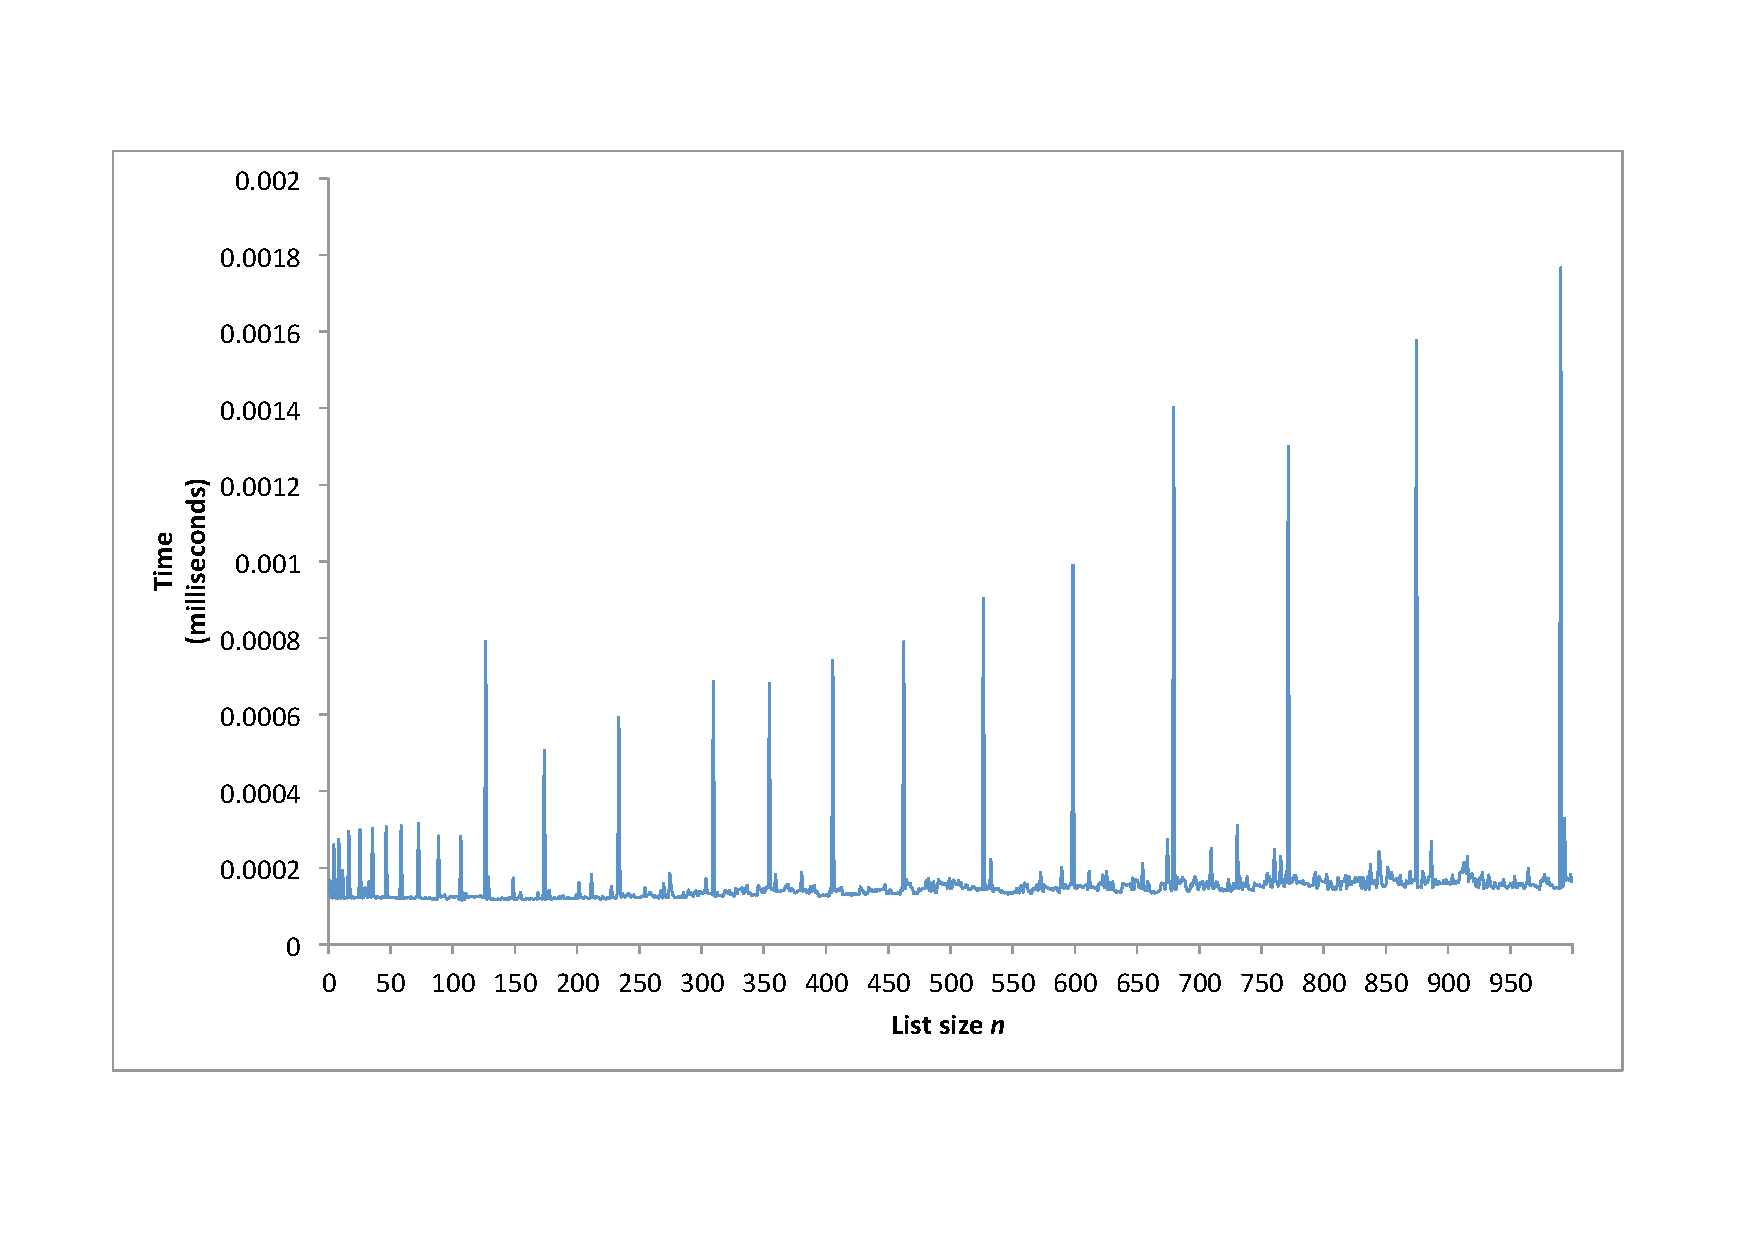
\includegraphics[height=0.9\textheight]{list_append_timing}
	\end{center}
\end{frame}

\begin{frame}{Operations on lists}
	\begin{itemize}
		\pause\item \textbf{Appending} to a list is \textbf{amortised constant time}
			\begin{itemize}
				\pause\item Usually $O(1)$, but can go up to $O(n)$ if the list needs to change size
			\end{itemize}
		\pause\item \textbf{Inserting} anywhere other than the end is \textbf{linear time}
			\begin{itemize}
				\pause\item Can't just insert new bytes into a memory block ---
					need to move all subsequent list elements to make room
			\end{itemize}
		\pause\item Similarly, \textbf{deleting} anything other than the last element is \textbf{linear time}
	\end{itemize}
\end{frame}

\begin{frame}{Tuples}
	\begin{itemize}
		\pause\item Tuples are like lists, but are \textbf{immutable}
			\begin{itemize}
				\pause\item Read-only
				\pause\item Once created, can't be changed
			\end{itemize}
		\pause\item Useful for storing sequences of values where adding, inserting, deleting or
			changing individual values does not make sense
			\begin{itemize}
				\pause\item E.g.\ $xy$ coordinates, RGB colours, ...
			\end{itemize}
		\pause\item Create tuples with \lstinline{()}, just as you create lists with \lstinline{[]}
			\begin{itemize}
				\pause\item Exception: a single element tuple is created as \lstinline{(foo,)}
					because \lstinline{(foo)} would be interpreted as a bracketed expression
			\end{itemize}
		\pause\item Can often omit the parentheses entirely, e.g.\ \lstinline{my_tuple = 1,2,3}
	\end{itemize}
\end{frame}

\begin{frame}[fragile]{Unpacking}
	If \lstinline{foo} is a list or tuple of length 4, the following are equivalent:
	\pause
	\begin{columns}
		\begin{column}{0.48\textwidth}
			\begin{lstlisting}
a, b, c, d = foo
			\end{lstlisting}
		\end{column}
		\pause
		\begin{column}{0.48\textwidth}
			\begin{lstlisting}
a = foo[0]
b = foo[1]
c = foo[2]
d = foo[3]
			\end{lstlisting}
		\end{column}
	\end{columns}
	\begin{itemize}
		\pause\item Unpacking requires the number of elements to match exactly ---
			if \lstinline{foo} has more than 4 elements, the code on the left will give an error
	\end{itemize}
\end{frame}

\begin{frame}[fragile]{One weird trick (Java programmers hate it!)}
	The following are equivalent:
	\pause
	\begin{columns}
		\begin{column}{0.48\textwidth}
			\begin{lstlisting}
a, b = b, a
			\end{lstlisting}
		\end{column}
		\pause
		\begin{column}{0.48\textwidth}
			\begin{lstlisting}
temp = a
a = b
b = temp
			\end{lstlisting}
		\end{column}
	\end{columns}
\end{frame}

\begin{frame}[fragile]{Strings are immutable}
	\begin{itemize}
		\pause\item \textbf{Strings} are immutable in Python
			\begin{itemize}
				\pause\item This is not true of all programming languages
			\end{itemize}
		\pause\item But wait... we change strings all the time, don't we?
	\end{itemize}
	\begin{lstlisting}
my_string = "Hello "
my_string += "world"
	\end{lstlisting}
	\begin{itemize}
		\pause\item This isn't changing the string, it's creating a new one and throwing the old one away!
		\pause\item Hence building a long string by appending can be slow (appending strings is $O(n)$)
	\end{itemize}
\end{frame}

\begin{frame}{Dictionaries}
	\begin{itemize}
		\pause\item Dictionaries are \textbf{associative maps}
		\pause\item A dictionary maps \textbf{keys} to \textbf{values}
			\begin{itemize}
				\pause\item Keys must be immutable (numbers, strings, tuples etc)
				\pause\item Values can be anything (including dictionaries or other containers)
			\end{itemize}
		\pause\item A dictionary is implemented as a \textbf{hash table}
	\end{itemize}		
\end{frame}

\begin{frame}[fragile]{Using dictionaries}
	\pause Create them using \lstinline|{}|:
	\begin{lstlisting}
age = {"Alice": 23, "Bob": 36, "Charlie": 27}
	\end{lstlisting}
	\pause Access values using \lstinline{[]}:
	\begin{lstlisting}
print(age["Alice"]) # prints 23
age["Bob"] = 40     # overwriting an existing item
age["Denise"] = 21  # adding a new item
	\end{lstlisting}
\end{frame}

\begin{frame}[fragile]{Iterating over dictionaries}
	\pause Iterating over a dictionary gives the \textbf{keys}:
	\begin{lstlisting}
for x in age:
    print(x)   # prints Alice, Bob, Charlie
	\end{lstlisting}
	\pause Use \lstinline{items} to get \textbf{key,value} pairs:
	\begin{lstlisting}
for key, value in age.items():
    print(key, "is", age, "years old")
	\end{lstlisting}
\end{frame}

\begin{frame}{Sets}
	\begin{itemize}
		\pause\item Sets are like dictionaries without the values
		\pause\item Sets are \textbf{unordered} collections of \textbf{unique} elements
            \begin{itemize}
                \pause\item Sets \textbf{cannot} contain \textbf{duplicate} elements
                \pause\item Attempting to \lstinline{add} an element already present in the set does nothing
            \end{itemize}
		\pause\item Certain operations on sets scale better on average than the equivalent operations on lists:
	\end{itemize}
	\pause
	\begin{center}
		\begin{tabular}{|c|c|c|}
			\hline
			\textbf{Operation} & \textbf{List} & \textbf{Set} \\\hline
			Add element & Append: $O(1)$ & $O(1)$ \\
			& Insert: $O(n)$ & \\\hline
			Delete element & $O(n)$ & $O(1)$ \\\hline
			Contains element? & $O(n)$ & $O(1)$ \\\hline
		\end{tabular}
	\end{center}
\end{frame}

\begin{frame}[fragile]{Using sets}
    \pause Create them using \lstinline|{}|:
	\begin{lstlisting}
numbers = {1, 4, 9, 16, 25}
	\end{lstlisting}
	\pause Add and remove members with \lstinline{add} and \lstinline{remove} methods
	\begin{lstlisting}
numbers.add(36)
numbers.remove(4)
	\end{lstlisting}
	\pause Test membership with \lstinline{in} operator
	\begin{lstlisting}
if 9 in numbers:
    print("Set contains 9")
	\end{lstlisting}
\end{frame}

\part{Basic data structures in C\#}
\frame{\partpage}

\begin{frame}{Classes and interfaces}
    \begin{itemize}
        \pause\item A \textbf{class} in C\# defines constructors, destructor, methods, properties, fields, ...
        \pause\item An \textbf{interface} defines methods and properties which a class can implement
        \pause\item An interface is a little like a fully abstract class
        \pause\item A class in C\# can only \textbf{inherit} from one \textbf{class},
            but can \textbf{implement} several \textbf{interfaces}
    \end{itemize}
\end{frame}

\begin{frame}{IEnumerable}
    \begin{itemize}
        \pause\item Most container types in C\# implement the \lstinline{IEnumerable<ElementType>} interface
        \pause\item Anything implementing \lstinline{IEnumerable} can be iterated over with a \lstinline{foreach} loop
    \end{itemize}
\end{frame}

\begin{frame}[fragile]{Arrays}
    \begin{lstlisting}
int[] myArray = new int[10];
int[] anotherArray = new int[] { 123, 456, 789 };
    \end{lstlisting}
    \begin{itemize}
        \pause\item \lstinline{int[]} is an array of \lstinline{int}s
        \pause\item Size of the array is set on initialisation with \lstinline{new}
        \pause\item Array \textbf{cannot change size} after initialisation
        \pause\item Use \lstinline{myArray[i]} to get/set the \lstinline{i}th element (starting at 0)
        \pause\item Use \lstinline{myArray.Length} to get the number of elements
    \end{itemize}
\end{frame}

\begin{frame}[fragile]{Multi-dimensional arrays}
    \begin{lstlisting}
int[,] myGrid = new int[20, 15];
    \end{lstlisting}
    \begin{itemize}
        \pause\item \lstinline{int[,]} is an 2-dimensional array of \lstinline{int}s
        \pause\item Use \lstinline{myArray[x, y]} to get/set elements
        \pause\item Use \lstinline{myArray.GetLength(0)}, \lstinline{myArray.GetLength(1)} to get the ``width'' and ``height''
        \pause\item Similarly \lstinline{int[,,]} is a 3-dimensional array, etc.
    \end{itemize}
\end{frame}

\begin{frame}[fragile]{Lists}
    \begin{lstlisting}
using System.Collections.Generic;

List<int> myList = new List<int>();
List<int> anotherList = new List<int> { 1, 2, 3, 4 };
    \end{lstlisting}
	\begin{itemize}
		\pause\item Like a list in Python, but can only store values of the specified type (here \lstinline{int})
		\pause\item Has similar time complexity properties to Python lists
		\pause\item Append elements with \lstinline{myList.Add()}
		\pause\item Get the number of elements with \lstinline{myList.Count}
	\end{itemize}
\end{frame}

\begin{frame}[fragile]{Strings}
    \begin{lstlisting}
string myString = "Hello, world!";
    \end{lstlisting}
	\begin{itemize}
		\pause\item \lstinline{string} can be thought of as a container
		\pause\item In particular, it implements \lstinline{IEnumerable<char>}
	\end{itemize}
\end{frame}

\begin{frame}[fragile]{Strings are immutable}
	\begin{itemize}
		\pause\item Strings are \textbf{immutable} in C\#
        \pause\item This is also true in Python, but not in all programming languages
		\pause\item But wait... we change strings all the time, don't we?
	\end{itemize}
	\begin{lstlisting}
string myString = "Hello ";
myString += "world";
	\end{lstlisting}
	\begin{itemize}
		\pause\item This isn't changing the string, it's creating a new one and throwing the old one away!
		\pause\item Hence building a long string by appending can be slow (appending strings is $O(n)$)
		\pause\item C\# has a \textbf{mutable} string type: \lstinline{StringBuilder}
	\end{itemize}
\end{frame}

\begin{frame}{Dictionaries}
	\begin{itemize}
		\pause\item Dictionaries are \textbf{associative maps}
		\pause\item A dictionary maps \textbf{keys} to \textbf{values}
		\pause\item Takes two generic parameters: the \textbf{key type} and the \textbf{value type}
		\pause\item A dictionary is implemented as a \textbf{hash table}
	\end{itemize}		
\end{frame}

\begin{frame}[fragile]{Using dictionaries}
	\begin{lstlisting}
var age = new Dictionary<string, int> {
    ["Alice"] = 23,
    ["Bob"] = 36,
    ["Charlie"] = 27
};
	\end{lstlisting}
	\pause Access values using \lstinline{[]}:
	\begin{lstlisting}
Console.WriteLine(age["Alice"]);  // prints 23
age["Bob"] = 40;      // overwriting an existing item
age["Denise"] = 21;   // adding a new item
age.Add("Emily", 29); // adding a new item -- error if already present
	\end{lstlisting}
\end{frame}

\begin{frame}[fragile]{Iterating over dictionaries}
	\begin{itemize}
		\pause\item \lstinline{Dictionary<Key, Value>} implements \lstinline{IEnumerable<KeyValuePair<Key, Value>>}
		\pause\item \lstinline{KeyValuePair<Key, Value>} stores \lstinline{Key} and \lstinline{Value}
	\end{itemize}		
	\pause
	\begin{lstlisting}
foreach (var kv in age)
{
    Console.WriteLine("{0} is {1} years old", kv.Key, kv.Value);
}
	\end{lstlisting}
	\begin{itemize}
	    \pause\item (Note the \lstinline{var} keyword --- automatically determines the appropriate type to use for a variable)
		\pause\item Dictionaries are \textbf{unordered} --- avoid assuming that \lstinline{foreach}
		    will see the elements in any particular order!
	\end{itemize}		
\end{frame}

\begin{frame}{Hash sets}
	\begin{itemize}
		\pause\item Sets are \textbf{unordered} collections of \textbf{unique} elements
            \begin{itemize}
                \pause\item Sets \textbf{cannot} contain \textbf{duplicate} elements
                \pause\item Attempting to \lstinline{Add} an element already present in the set does nothing
            \end{itemize}
		\pause\item \lstinline{HashSet}s are like \lstinline{Dictionary}s without the values, just the keys
		\pause\item Certain operations on sets scale better on average than the equivalent operations on lists:
	\end{itemize}
	\pause
	\begin{center}
		\begin{tabular}{|c|c|c|}
			\hline
			\textbf{Operation} & \textbf{List} & \textbf{Hash Set} \\\hline
			Add element & Append: $O(1)$ & $O(1)$ \\
			& Insert: $O(n)$ & \\\hline
			Delete element & $O(n)$ & $O(1)$ \\\hline
			Contains element? & $O(n)$ & $O(1)$ \\\hline
		\end{tabular}
	\end{center}
\end{frame}

\begin{frame}[fragile]{Using sets}
	\begin{lstlisting}
var numbers = new HashSet<int>{1, 4, 9, 16, 25};
	\end{lstlisting}
	\pause Add and remove members with \lstinline{Add} and \lstinline{Remove} methods
	\begin{lstlisting}
numbers.Add(36);
numbers.Remove(4);
	\end{lstlisting}
	\pause Test membership with \lstinline{Contains}
	\begin{lstlisting}
if (numbers.Contains(9))
    Console.WriteLine("Set contains 9");
	\end{lstlisting}
\end{frame}

\part{More data structures}
\frame{\partpage}

\begin{frame}{Stacks and queues}
	\begin{columns}
		\pause
		\begin{column}{0.3\textwidth}
			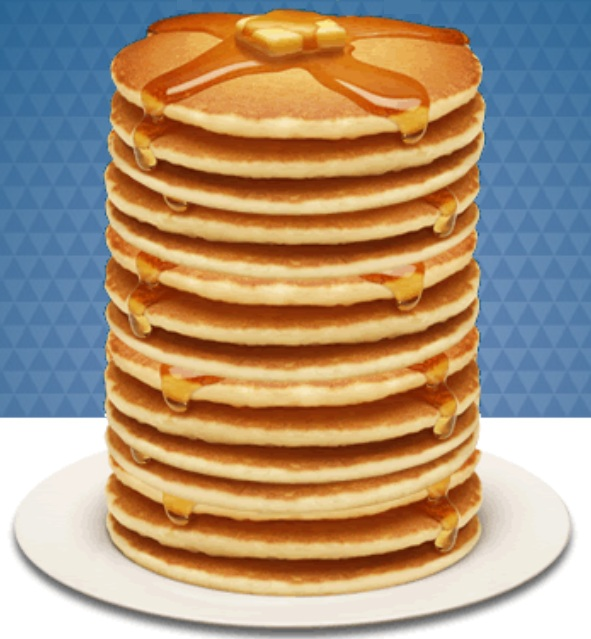
\includegraphics[width=\textwidth]{stack}
		\end{column}
		\begin{column}{0.68\textwidth}
			\begin{itemize}
				\item A \textbf{stack} is a \textbf{last-in first-out (LIFO)} data structure
				\pause\item Items can be \textbf{pushed} to the \textbf{top} of the stack
				\pause\item Items can be \textbf{popped} from the \textbf{top} of the stack
			\end{itemize}
		\end{column}
	\end{columns}
	\begin{columns}
		\pause
		\begin{column}{0.3\textwidth}
			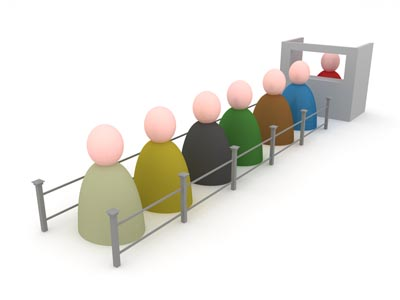
\includegraphics[width=\textwidth]{queue}
		\end{column}
		\begin{column}{0.68\textwidth}
			\begin{itemize}
				\item A \textbf{queue} is a \textbf{first-in first-out (LIFO)} data structure
				\pause\item Items can be \textbf{enqueued} to the \textbf{back} of the queue
				\pause\item Items can be \textbf{dequeued} from the \textbf{front} of the queue
			\end{itemize}
		\end{column}
	\end{columns}
\end{frame}

\begin{frame}{Stacks and queues in Python}
	\begin{itemize}
		\pause\item Stacks can be implemented efficiently as lists
		\pause\item Queues can be implemented as lists, but not efficiently
		\pause\item \lstinline{deque} (from the \lstinline{collections} module) implements an efficient
			\textbf{double-ended queue}
		\pause\item Inserting and removing elements from the start and end of a \lstinline{deque} is $O(1)$
	\end{itemize}
\end{frame}

\begin{frame}{Graphs}
	\begin{columns}
		\pause
		\begin{column}{0.3\textwidth}
			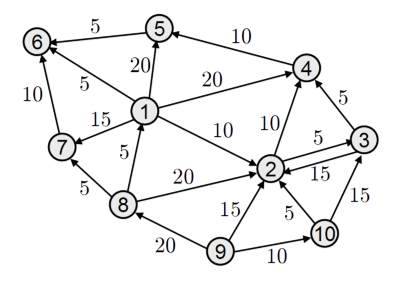
\includegraphics[width=\textwidth]{graph1}
			\par
			\vspace{2ex}
			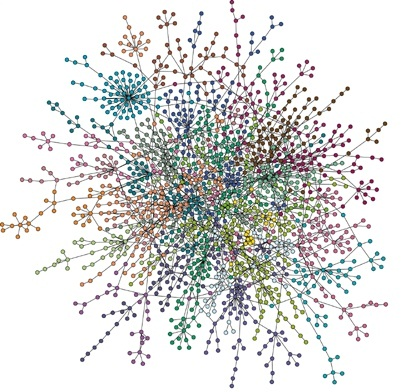
\includegraphics[width=\textwidth]{graph2}
		\end{column}
		\begin{column}{0.68\textwidth}
			\begin{itemize}
				\pause\item A \textbf{graph} is defined by:
					\begin{itemize}
						\pause\item A collection of \textbf{nodes} or \textbf{vertices} (points)
						\pause\item A collection of \textbf{edges} or \textbf{arcs} (undirected lines or directed arrows between points)
					\end{itemize}
				\pause\item Often used to model \textbf{networks} (e.g.\ social networks, transport networks, game levels, finite state automata, ...)
			\end{itemize}
		\end{column}
	\end{columns}
\end{frame}

\begin{frame}{Trees}
	\begin{columns}
		\pause
		\begin{column}{0.3\textwidth}
			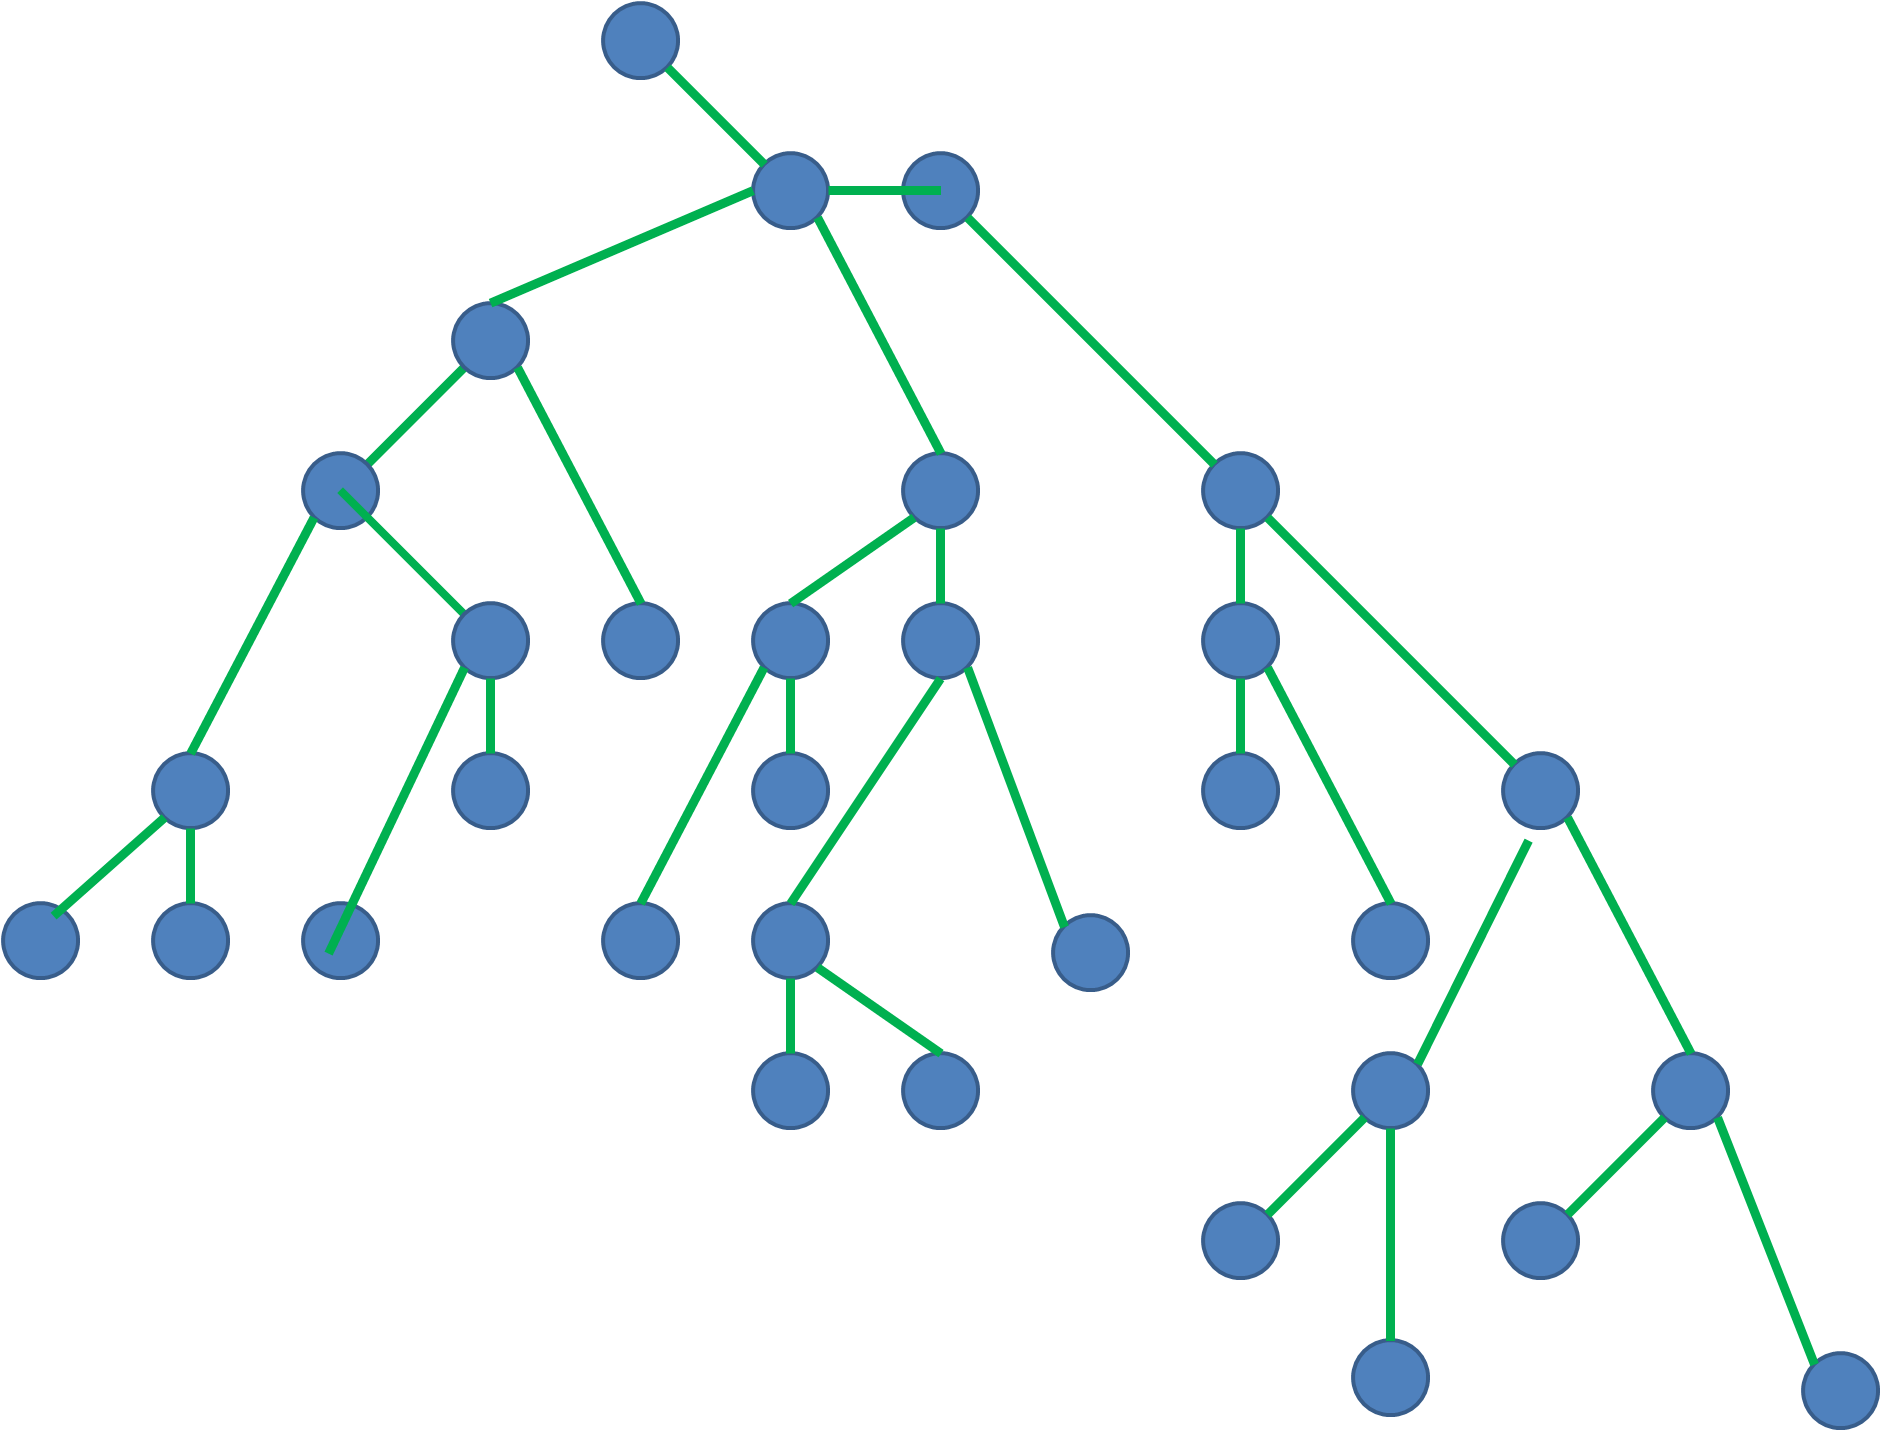
\includegraphics[width=\textwidth]{tree2}
			\par
			\vspace{2ex}
			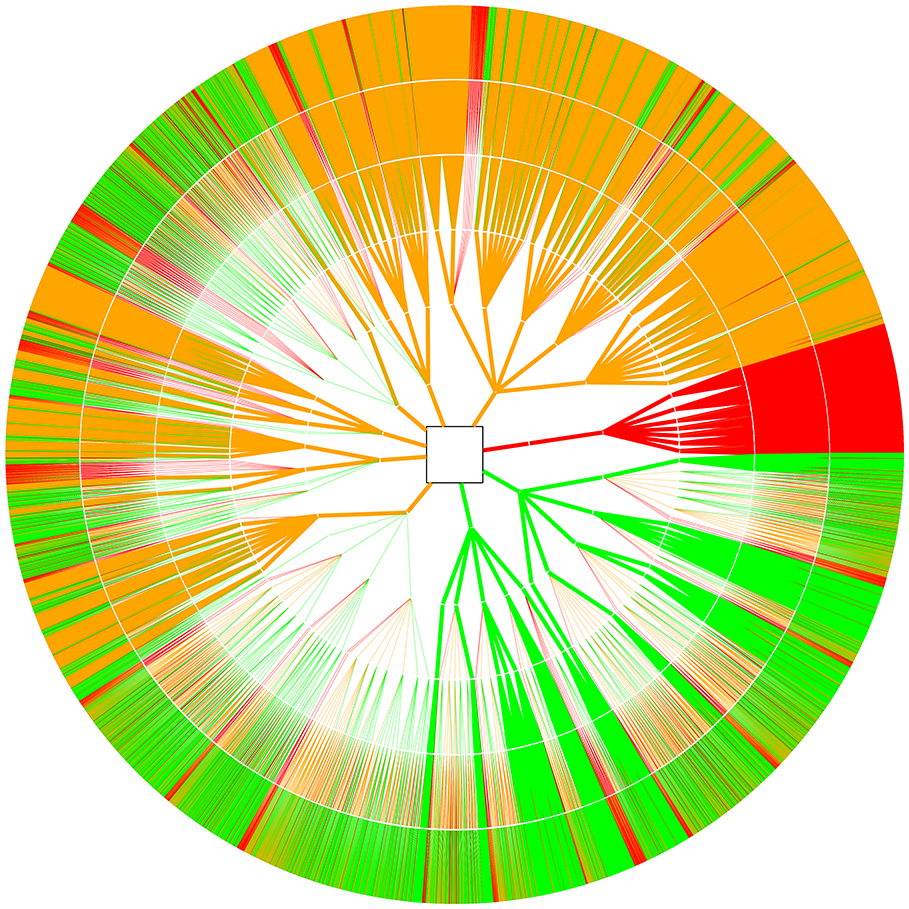
\includegraphics[width=\textwidth]{tree}
		\end{column}
		\begin{column}{0.68\textwidth}
			\begin{itemize}
				\pause\item A \textbf{tree} is a special type of directed graph where:
					\begin{itemize}
						\pause\item One node (the \textbf{root}) has no incoming edges
						\pause\item All other nodes have exactly 1 incoming edge
					\end{itemize}
				\pause\item Edges go from \textbf{parent} to \textbf{child}
					\begin{itemize}
						\pause\item All nodes except the root have exactly one parent
						\pause\item Nodes can have 0, 1 or many children
					\end{itemize}
				\pause\item Used to model \textbf{hierarchies} (e.g.\ file systems, object inheritance, scene graphs, state-action trees, ...)
			\end{itemize}
		\end{column}
	\end{columns}
\end{frame}



% \part{Workshop time}
% \frame{\partpage}

% \begin{frame}{Workshop}
%     \begin{itemize}
%         \item Continue working on your \textbf{research journal} to prepare for the peer review on Thursday
%         \item Today, pay particular attention to your \textbf{bibliography}
%         \item Common pitfalls to watch out for:
%         \begin{itemize}
%             \item Do entries have all required fields?
%             \item Are proper nouns etc in titles correctly capitalised?
%             \item Are names with accented characters properly formatted?
%             \item Are there duplicate entries?
%         \end{itemize}
%         \item Feel free to use your breakout groups (from previous weeks) to check each other's bibliographies over and help each other fix any issues
%         \item Post in chat here if you have questions or problems!
%     \end{itemize}
% \end{frame}

\end{document}
